\documentclass{article}
% Adjust the relative path to point to the latex-templates directory
% Absolute paths for template files

% content/resources/templates/preamble.tex
\usepackage[margin=0.6in]{geometry}
\author{Milav Dabgar}
\usepackage{amsmath,amssymb,amsthm}
\usepackage{booktabs}
\usepackage{multirow}
\usepackage{xcolor}
\usepackage{tcolorbox}
\tcbuselibrary{breakable,skins}
\usepackage[colorlinks=true,linkcolor=blue]{hyperref}
\usepackage{titlesec}
\usepackage{enumitem}
\usepackage{tikz}
\usepackage{pgfplots}
\usepackage{circuitikz}
\usepackage[version=4]{mhchem}
\usepackage{longtable}
\usepackage{array}
\usepackage{float}
\usepackage{caption}
\usepackage{listings}

\lstset{
  basicstyle=\small\ttfamily,
  breaklines=true,
  breakatwhitespace=false,
  postbreak=\mbox{\textcolor{red}{$\hookrightarrow$}\space},
  float=false,
  numbers=left,
  numberstyle=\tiny\color{gray},
  numbersep=10pt,
  xleftmargin=2em,
  keywordstyle=\color{blue},
  commentstyle=\color{green!60!black},
  stringstyle=\color{purple},
  backgroundcolor=\color{gray!5},
  showstringspaces=false,
  tabsize=2,
  captionpos=b,
  keepspaces=true,
  columns=flexible
}

\pgfplotsset{compat=1.18}
\usetikzlibrary{shapes,arrows,positioning,calc,patterns,decorations.pathmorphing,decorations.markings,arrows.meta}

% Color scheme
\definecolor{headcolor}{RGB}{0,102,204}
\definecolor{keycolor}{RGB}{220,20,60}
\definecolor{solutioncolor}{RGB}{34,139,34}
\definecolor{mnemoniccolor}{RGB}{148,0,211}
\definecolor{codecolor}{RGB}{0,0,100}

% Spacing
\setlength{\parskip}{3pt}
\setlist[itemize]{nosep}
\setlist[enumerate]{nosep}

% Title formatting
\titleformat{\section}{\Large\bfseries\color{headcolor}}{\thesection}{1em}{}
\titleformat{\subsection}{\large\bfseries\color{headcolor}}{\thesubsection}{1em}{}

% Pandoc tightlist compatibility
\providecommand{\tightlist}{%
  \setlength{\itemsep}{0pt}\setlength{\parskip}{0pt}}

% Pandoc longtable compatibility
\newcounter{none}
\def\thenone{}


% content/resources/templates/english-boxes.tex

% Custom environments
\newtcolorbox{solutionbox}{
 breakable,
 enhanced,
 colback=solutioncolor!5!white,
 colframe=solutioncolor!75!black,
 fonttitle=\bfseries,
 title=Solution
}

\newtcolorbox{solutionboxnobreak}{
 colback=solutioncolor!5!white,
 colframe=solutioncolor!75!black,
 fonttitle=\bfseries,
 title=Solution
}

\newtcolorbox{keyformula}{
 breakable,
 enhanced,
 colback=keycolor!5!white,
 colframe=keycolor!75!black,
 fonttitle=\bfseries,
 title=Key Formula
}

\newtcolorbox{mnemonicboxenv}{
 breakable,
 enhanced,
 colback=mnemoniccolor!5!white,
 colframe=mnemoniccolor!75!black,
 fonttitle=\bfseries,
 title=Mnemonic
}

\newcommand{\mnemonicbox}[1]{%
  \begin{mnemonicboxenv}
    #1
  \end{mnemonicboxenv}
}


% Custom commands for GTU solutions
% This file defines semantic commands for consistent formatting

% Question command with automatic formatting
\newcommand{\question}[2]{%
  \section*{Question #1}%
  \textbf{#2}%
}

% OR question variant
\newcommand{\questionor}[2]{%
  \section*{Question #1 OR}%
  \textbf{#2}%
}

% Proper table environment with caption
\newenvironment{answertable}[1]{%
  \begin{table}[htbp]
  \centering
  \caption{#1}
}{%
  \end{table}
}

% Proper figure environment for diagrams
\newenvironment{answerdiagram}[1]{%
  \begin{figure}[htbp]
  \centering
  \caption{#1}
}{%
  \end{figure}
}

% Semantic markup for key terms
\newcommand{\keyword}[1]{\textbf{#1}}
\newcommand{\code}[1]{\texttt{#1}}
\newcommand{\classname}[1]{\texttt{#1}}
\newcommand{\methodname}[1]{\texttt{#1}}

% Proper quotation marks
\newcommand{\mnemonic}[1]{``#1''}


\title{Communication Engineering (1333201) - Winter 2024 Solution}
\date{May 19, 2024}

\begin{document}
\maketitle

\questionmarks{1(a)}{3}{What is modulation? What is the need of it?}

\begin{solutionbox}
Modulation is the process of varying one or more properties of a high-frequency carrier signal with a modulating signal containing information.

\begin{center}
\captionof{table}{Need for Modulation}
\begin{tabulary}{\linewidth}{|L|L|}
\hline
\textbf{Reason} & \textbf{Explanation} \\ \hline
Antenna Size & Reduces antenna size requirements ($\lambda = c/f$) \\ \hline
Multiplexing & Allows multiple signals to share the spectrum \\ \hline
Range & Increases transmission distance \\ \hline
Interference & Reduces noise interference \\ \hline
\end{tabulary}
\end{center}

\begin{itemize}
    \item \textbf{Practical transmission}: Makes low-frequency information signals suitable for wireless transmission
    \item \textbf{Signal separation}: Enables different signals to be transmitted simultaneously
\end{itemize}
\end{solutionbox}

\begin{mnemonicbox}
\mnemonic{RARE Messages: Range, Antenna, Reduce interference, Enable multiplexing}
\end{mnemonicbox}

\begin{center}
\begin{tikzpicture}[node distance=1.5cm, auto, >=latex, thick]
    \node [gtu block] (source) {Information\\Source};
    \node [gtu block, right=1.5cm of source] (mod) {Modulator};
    \node [gtu block, right=1.5cm of mod] (chan) {Channel};
    \node [gtu block, right=1.5cm of chan] (demod) {Demodulator};
    \node [gtu block, right=1.5cm of demod] (dest) {Destination};
    
    \node [above=0.5cm of mod] (carrier) {Carrier};
    \draw [gtu arrow] (carrier) -- (mod);
    
    \draw [gtu arrow] (source) -- (mod);
    \draw [gtu arrow] (mod) -- (chan);
    \draw [gtu arrow] (chan) -- (demod);
    \draw [gtu arrow] (demod) -- (dest);
    
    \node [above of=chan, node distance=1.5cm] (noise) {Noise};
    \draw [gtu arrow] (noise) -- (chan);
\end{tikzpicture}
\captionof{figure}{Communication System Block Diagram}
\end{center}

\questionmarks{1(b)}{4}{Compare AM and FM.}

\begin{solutionbox}
\begin{center}
\captionof{table}{Comparison between AM and FM}
\begin{tabulary}{\linewidth}{|L|L|L|}
\hline
\textbf{Parameter} & \textbf{AM (Amplitude Modulation)} & \textbf{FM (Frequency Modulation)} \\ \hline
Parameter varied & Amplitude of carrier & Frequency of carrier \\ \hline
Bandwidth & Narrow ($2 \times f_m$) & Wide ($2 \times (m_f + 1) f_m$) \\ \hline
Noise immunity & Poor & Excellent \\ \hline
Power efficiency & Less efficient & More efficient \\ \hline
Circuit complexity & Simple & Complex \\ \hline
Quality & Moderate & High \\ \hline
Applications & Medium wave broadcasting & High-fidelity broadcasting \\ \hline
\end{tabulary}
\end{center}
\end{solutionbox}

\begin{mnemonicbox}
\mnemonic{BANC-QA: Bandwidth, Amplitude/frequency, Noise, Complexity, Quality, Applications}
\end{mnemonicbox}

\questionmarks{1(c)}{7}{Explain Amplitude modulation with waveform and derive voltage equation for modulated signal also Sketch the frequency spectrum of the DSBFC AM.}

\begin{solutionbox}
Amplitude Modulation (AM) is a technique where the amplitude of a carrier wave is varied in proportion to the instantaneous amplitude of the modulating signal.

\textbf{Voltage Equation:}

\begin{itemize}
    \item Carrier signal: $v_1(t) = A_1 \sin(\omega_c t)$
    \item Modulating signal: $v_2(t) = A_2 \sin(\omega_m t)$
    \item Modulated signal: $v(t) = A_1[1 + m \sin(\omega_m t)] \sin(\omega_c t)$
    \item Where $m = A_2/A_1$ (modulation index)
\end{itemize}

\begin{center}
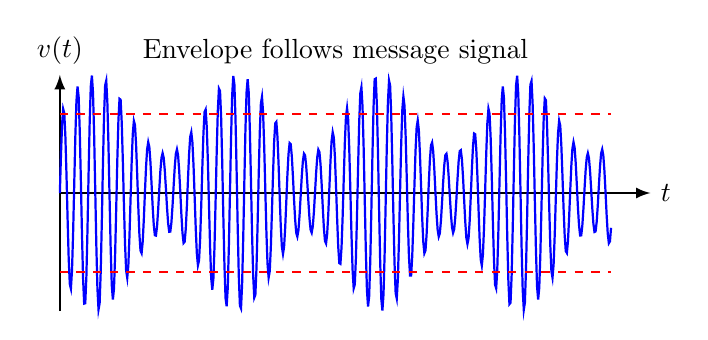
\begin{tikzpicture}[x=0.05cm,y=1.0cm, >=latex, thick]
    % Axes
    \draw[->] (0,0) -- (150,0) node[right] {$t$};
    \draw[->] (0,-1.5) -- (0,1.5) node[above] {$v(t)$};
    
    % Waveform
    \draw[blue, domain=0:140, samples=500] plot (\x, {(1 + 0.5*sin(10*\x)) * sin(100*\x)});
    \draw[dashed, red] (0,1) -- (140,1);
    \draw[dashed, red] (0,-1) -- (140,-1);
    
    \node at (70, 1.8) {Envelope follows message signal};
\end{tikzpicture}
\captionof{figure}{AM Waveform}
\end{center}

\textbf{Frequency Spectrum of DSBFC AM}

\begin{center}
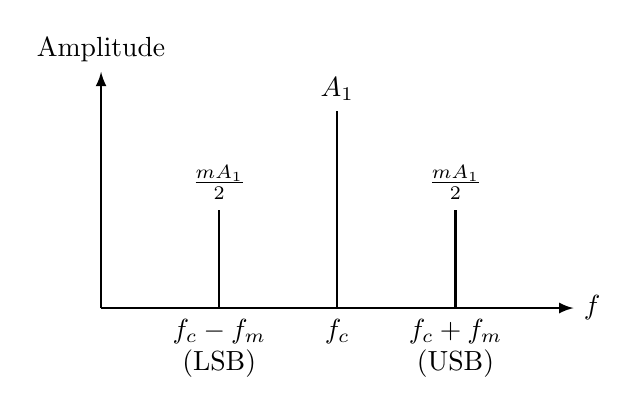
\begin{tikzpicture}[>=latex, thick]
    \draw[->] (0,0) -- (6,0) node[right] {$f$};
    \draw[->] (0,0) -- (0,3) node[above] {Amplitude};
    
    \draw[thick] (3,0) -- (3,2.5) node[above] {$A_1$};
    \node at (3,-0.3) {$f_c$};
    
    \draw[thick] (1.5,0) -- (1.5,1.25) node[above] {$\frac{mA_1}{2}$};
    \node at (1.5,-0.3) {$f_c - f_m$};
    \node at (1.5,-0.7) {(LSB)};
    
    \draw[thick] (4.5,0) -- (4.5,1.25) node[above] {$\frac{mA_1}{2}$};
    \node at (4.5,-0.3) {$f_c + f_m$};
    \node at (4.5,-0.7) {(USB)};
\end{tikzpicture}
\captionof{figure}{AM Frequency Spectrum}
\end{center}

\begin{itemize}
    \item \textbf{Bandwidth}: The bandwidth of AM signal is $2 \times f_m$
    \item \textbf{Sidebands}: Upper sideband (USB) at $f_c+f_m$ and Lower sideband (LSB) at $f_c-f_m$
    \item \textbf{Power distribution}: In carrier and two sidebands
\end{itemize}
\end{solutionbox}

\begin{mnemonicbox}
\mnemonic{CAM-SIP: Carrier Amplitude Modified, Sidebands In Pair}
\end{mnemonicbox}

\questionmarks{1(c OR)}{7}{Derive the equation for total power in AM, calculate percentage of power savings in DSB and SSB.}

\begin{solutionbox}
\textbf{Derivation of Total Power in AM:}

\begin{itemize}
    \item AM signal: $v(t) = A_1[1 + m \sin(\omega_m t)] \sin(\omega_c t)$
    \item Total power: $P = P_{\text{carrier}} + P_{\text{sidebands}}$
    \item $P_{\text{carrier}} = A_1^2/2$
    \item $P_{\text{sidebands}} = A_1^2 m^2/4$
\end{itemize}

\begin{center}
\captionof{table}{Power Distribution in AM}
\begin{tabulary}{\linewidth}{|L|L|L|}
\hline
\textbf{Component} & \textbf{Power Expression} & \textbf{\% of Total Power (m=1)} \\ \hline
Carrier & $P_c = A_1^2/2$ & 66.67\% \\ \hline
Sidebands & $P_s = A_1^2 m^2/4$ & 33.33\% \\ \hline
Total & $P_t = A_1^2(1+m^2/2)/2$ & 100\% \\ \hline
\end{tabulary}
\end{center}

\textbf{Power Savings:}

\begin{itemize}
    \item \textbf{DSB-SC}: 100\% carrier power saved (66.67\% of total power)
    \begin{itemize}
        \item Only sidebands are transmitted
        \item Percentage savings = $(P_c/P_t) \times 100 = 66.67\%$
    \end{itemize}
    
    \item \textbf{SSB}: 50\% of sideband power + 100\% carrier power saved
    \begin{itemize}
        \item One sideband + carrier removed
        \item Percentage savings = $(P_c + P_s/2)/P_t \times 100 = 83.33\%$
    \end{itemize}
\end{itemize}
\end{solutionbox}

\begin{mnemonicbox}
\mnemonic{CAST-83: Carrier And Sideband Transmission, 83\% saved in SSB}
\end{mnemonicbox}

\questionmarks{2(a)}{3}{Define (1) Modulation index for AM (2) Modulation index For FM.}

\begin{solutionbox}
\begin{center}
\captionof{table}{Modulation Index Definitions}
\begin{tabulary}{\linewidth}{|L|L|L|}
\hline
\textbf{Parameter} & \textbf{AM Modulation Index} & \textbf{FM Modulation Index} \\ \hline
Definition & Ratio of peak amplitude of modulating signal to peak amplitude of carrier & Ratio of frequency deviation to modulating frequency \\ \hline
Formula & $m = A_m/A_c$ & $m_f = \Delta f/f_m$ \\ \hline
Range & $0 \le m \le 1$ for no distortion & No specific upper limit \\ \hline
Effect & Determines \% modulation & Determines bandwidth \\ \hline
\end{tabulary}
\end{center}

\begin{itemize}
    \item \textbf{AM Modulation Index}: Controls the amplitude variation and power distribution
    \item \textbf{FM Modulation Index}: Determines bandwidth and signal quality
\end{itemize}
\end{solutionbox}

\begin{mnemonicbox}
\mnemonic{ARM-FDM: Amplitude Ratio for Modulation, Frequency Deviation for Modulation}
\end{mnemonicbox}

\questionmarks{2(b)}{4}{Draw and explain block diagram for envelope detector.}

\begin{solutionbox}
\begin{center}
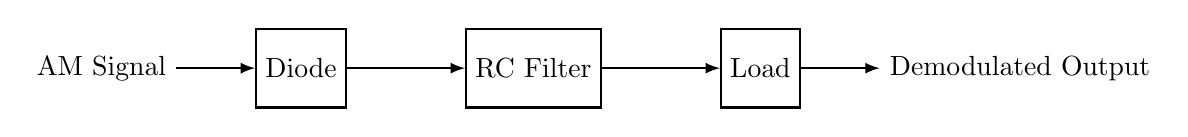
\begin{tikzpicture}[auto, >=latex, thick, node distance=1.5cm]
    \node (input) {AM Signal};
    \node [draw, rectangle, minimum size=1cm, right=1cm of input] (diode) {Diode};
    \node [draw, rectangle, minimum size=1cm, right=1.5cm of diode] (rc) {RC Filter};
    \node [draw, rectangle, minimum size=1cm, right=1.5cm of rc] (load) {Load};
    \node [right=1cm of load] (output) {Demodulated Output};
    
    \draw [->] (input) -- (diode);
    \draw [->] (diode) -- (rc);
    \draw [->] (rc) -- (load);
    \draw [->] (load) -- (output);
\end{tikzpicture}
\captionof{figure}{Envelope Detector Block Diagram}
\end{center}

\begin{center}
\captionof{table}{Components and Their Functions}
\begin{tabulary}{\linewidth}{|L|L|}
\hline
\textbf{Component} & \textbf{Function} \\ \hline
Diode & Rectifies the AM signal (removes negative half-cycles) \\ \hline
RC Filter & Smooths the rectified signal to recover the envelope \\ \hline
Load & Provides output circuit and impedance matching \\ \hline
\end{tabulary}
\end{center}

\begin{itemize}
    \item \textbf{Working principle}: The diode conducts only during positive half-cycles
    \item \textbf{Time constant}: RC must be large enough to prevent ripple but small enough to follow modulation
    \item \textbf{Condition}: $RC \gg 1/f_c$ but $RC \ll 1/f_m$
\end{itemize}
\end{solutionbox}

\begin{mnemonicbox}
\mnemonic{DEER: Diode Extracts Envelope Representation}
\end{mnemonicbox}

\questionmarks{2(c)}{7}{Draw block diagram of FM radio receiver and explain working of each block.}

\begin{solutionbox}
\begin{center}
\begin{tikzpicture}[node distance=1.5cm, auto, >=latex, thick, scale=0.8, transform shape]
    \node [gtu block] (ant) {Antenna};
    \node [gtu block, right=1cm of ant] (rf) {RF Amplifier};
    \node [gtu block, right=1cm of rf] (mix) {Mixer};
    \node [gtu block, below=1cm of mix] (lo) {Local Oscillator};
    \node [gtu block, right=1cm of mix] (if) {IF Amplifier};
    \node [gtu block, right=1cm of if] (lim) {Limiter};
    \node [gtu block, below=1cm of lim] (disc) {FM Discriminator};
    \node [gtu block, left=1cm of disc] (audio) {Audio Amplifier};
    \node [gtu block, left=1cm of audio] (spk) {Speaker};
    
    \draw [gtu arrow] (ant) -- (rf);
    \draw [gtu arrow] (rf) -- (mix);
    \draw [gtu arrow] (lo) -- (mix);
    \draw [gtu arrow] (mix) -- (if);
    \draw [gtu arrow] (if) -- (lim);
    \draw [gtu arrow] (lim) -- (disc);
    \draw [gtu arrow] (disc) -- (audio);
    \draw [gtu arrow] (audio) -- (spk);
\end{tikzpicture}
\captionof{figure}{FM Radio Receiver}
\end{center}

\begin{center}
\captionof{table}{Functions of Each Block}
\begin{tabulary}{\linewidth}{|L|L|}
\hline
\textbf{Block} & \textbf{Function} \\ \hline
Antenna & Receives electromagnetic waves \\ \hline
RF Amplifier & Amplifies weak RF signals (88-108 MHz) \\ \hline
Mixer & Converts RF to IF frequency (10.7 MHz) \\ \hline
Local Oscillator & Generates frequency for mixing (RF+10.7 MHz) \\ \hline
IF Amplifier & Amplifies IF signal with fixed gain \\ \hline
Limiter & Removes amplitude variations \\ \hline
FM Discriminator & Converts frequency variations to voltage \\ \hline
Audio Amplifier & Amplifies recovered audio \\ \hline
Speaker & Converts electrical to sound waves \\ \hline
\end{tabulary}
\end{center}

\begin{itemize}
    \item \textbf{Superheterodyne principle}: Uses frequency conversion to process signals at fixed IF
    \item \textbf{Distinctive FM feature}: Limiter removes noise in amplitude before demodulation
\end{itemize}
\end{solutionbox}

\begin{mnemonicbox}
\mnemonic{RAMLIDASS: RF, Amplifier, Mixer, Local oscillator, IF, Discriminator, Audio, Speaker System}
\end{mnemonicbox}

\questionmarks{2(a OR)}{3}{Draw only Waveform For frequency modulation and Phase modulation.}

\begin{solutionbox}
\begin{center}
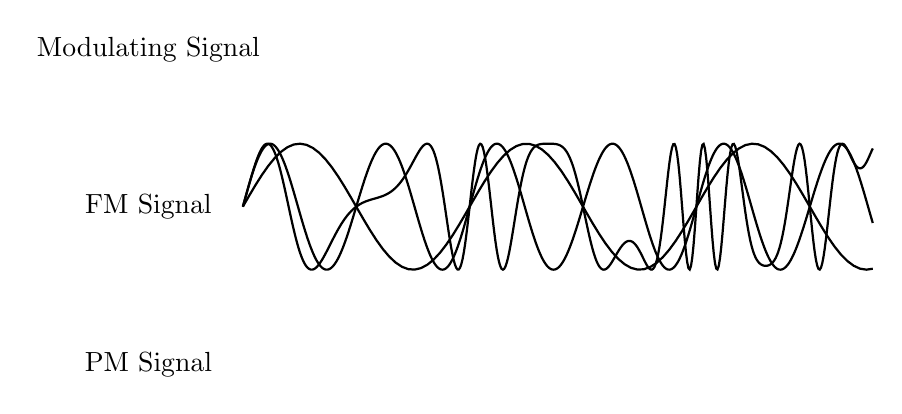
\begin{tikzpicture}[x=0.08cm,y=0.8cm, >=latex, thick]
    \node at (-15, 2.5) {Modulating Signal};
    \draw[domain=0:100, samples=100] plot (\x, {sin(10*\x)});
    
    \node at (-15, 0) {FM Signal};
    \draw[domain=0:100, samples=500] plot (\x, {sin((20 + 5*sin(10*\x))*\x)});
    
    \node at (-15, -2.5) {PM Signal};
    \draw[domain=0:100, samples=500] plot (\x, {sin(20*\x + 5*sin(10*\x))});
\end{tikzpicture}
\captionof{figure}{FM and PM Waveforms}
\end{center}

\textbf{Key Characteristics:}

\begin{itemize}
    \item \textbf{FM}: Frequency increases when modulating signal is positive
    \item \textbf{PM}: Phase shifts immediately with amplitude changes
\end{itemize}
\end{solutionbox}

\begin{mnemonicbox}
\mnemonic{FIP-PAF: Frequency Increases with Positive signal, Phase Advances with Faster changes}
\end{mnemonicbox}

\questionmarks{2(b OR)}{4}{Define any FOUR characteristics of radio receiver.}

\begin{solutionbox}
\begin{center}
\captionof{table}{Characteristics of Radio Receiver}
\begin{tabulary}{\linewidth}{|L|L|}
\hline
\textbf{Characteristic} & \textbf{Definition} \\ \hline
Sensitivity & Ability to receive weak signals (measured in $\mu$V or dBm) \\ \hline
Selectivity & Ability to separate desired signal from adjacent channels \\ \hline
Fidelity & Accuracy of reproducing the original modulating signal \\ \hline
Image Rejection & Ability to reject image frequency interference \\ \hline
\end{tabulary}
\end{center}

\textbf{Additional characteristics:}

\begin{itemize}
    \item \textbf{Signal-to-Noise Ratio}: Ratio of signal power to noise power
    \item \textbf{Bandwidth}: Range of frequencies that can be received
    \item \textbf{Stability}: Ability to maintain tuned frequency
\end{itemize}
\end{solutionbox}

\begin{mnemonicbox}
\mnemonic{SFIS-BSS: Sensitivity, Fidelity, Image rejection, Selectivity - Better Signal Stability}
\end{mnemonicbox}

\questionmarks{2(c OR)}{7}{Draw block diagram of AM radio receiver and explain working of each block.}

\begin{solutionbox}
\begin{center}
\begin{tikzpicture}[node distance=1.5cm, auto, >=latex, thick, scale=0.8, transform shape]
    \node [gtu block] (ant) {Antenna};
    \node [gtu block, right=1cm of ant] (rf) {RF Tuner \&\\Amplifier};
    \node [gtu block, right=1cm of rf] (mix) {Mixer};
    \node [gtu block, below=1cm of mix] (lo) {Local\\Oscillator};
    \node [gtu block, right=1cm of mix] (if) {IF\\Amplifier};
    \node [gtu block, right=1cm of if] (det) {Detector};
    \node [gtu block, below=1cm of det] (agc) {AGC};
    \node [gtu block, right=1cm of det] (audio) {Audio\\Amplifier};
    \node [gtu block, right=1cm of audio] (spk) {Speaker};
    
    \draw [gtu arrow] (ant) -- (rf);
    \draw [gtu arrow] (rf) -- (mix);
    \draw [gtu arrow] (lo) -- (mix);
    \draw [gtu arrow] (mix) -- (if);
    \draw [gtu arrow] (if) -- (det);
    \draw [gtu arrow] (det) -- (audio);
    \draw [gtu arrow] (det) -- (agc);
    \draw [gtu arrow] (agc) -| (if);
    \draw [gtu arrow] (audio) -- (spk);
\end{tikzpicture}
\captionof{figure}{AM Radio Receiver}
\end{center}

\begin{center}
\captionof{table}{Functions of Each Block}
\begin{tabulary}{\linewidth}{|L|L|}
\hline
\textbf{Block} & \textbf{Function} \\ \hline
Antenna & Captures AM radio waves \\ \hline
RF Tuner \& Amplifier & Selects and amplifies desired frequency \\ \hline
Mixer & Converts RF signal to IF (455 kHz) \\ \hline
Local Oscillator & Generates frequency for mixing (RF+455 kHz) \\ \hline
IF Amplifier & Amplifies IF signal with fixed selectivity \\ \hline
Detector & Recovers audio from AM envelope \\ \hline
AGC & Provides automatic gain control \\ \hline
Audio Amplifier & Amplifies audio signal \\ \hline
Speaker & Converts electrical to sound waves \\ \hline
\end{tabulary}
\end{center}

\begin{itemize}
    \item \textbf{Superheterodyne principle}: Uses frequency conversion for better selectivity
    \item \textbf{AGC feedback loop}: Maintains constant output despite signal strength variations
\end{itemize}
\end{solutionbox}

\begin{mnemonicbox}
\mnemonic{ARMLESS: Antenna, RF, Mixer, Local oscillator, Envelope detector, Sound System}
\end{mnemonicbox}


\questionmarks{3(a)}{3}{Define quantization. Explain non uniform quantization in brief.}

\begin{solutionbox}
\textbf{Quantization} is the process of converting continuous amplitude values into discrete levels for digital representation.

\begin{center}
\captionof{table}{Non-uniform Quantization}
\begin{tabulary}{\linewidth}{|L|L|}
\hline
\textbf{Aspect} & \textbf{Description} \\ \hline
Definition & Assigning different step sizes for different amplitude ranges \\ \hline
Advantage & Reduces quantization noise for small amplitude signals \\ \hline
Implementation & Using companding (compression-expansion) techniques \\ \hline
Example & $\mu$-law and A-law companding used in telephony \\ \hline
\end{tabulary}
\end{center}

\begin{itemize}
    \item \textbf{Working principle}: Smaller step sizes for lower amplitudes, larger steps for higher amplitudes
    \item \textbf{Effect}: Improves SNR for weak signals at the expense of strong signals
\end{itemize}
\end{solutionbox}

\begin{mnemonicbox}
\mnemonic{QUEST-CS: QUantization with Enhanced Steps - Compressing Small signals}
\end{mnemonicbox}

\questionmarks{3(b)}{4}{Explain Sample and hold Circuit with Waveform.}

\begin{solutionbox}
\begin{center}
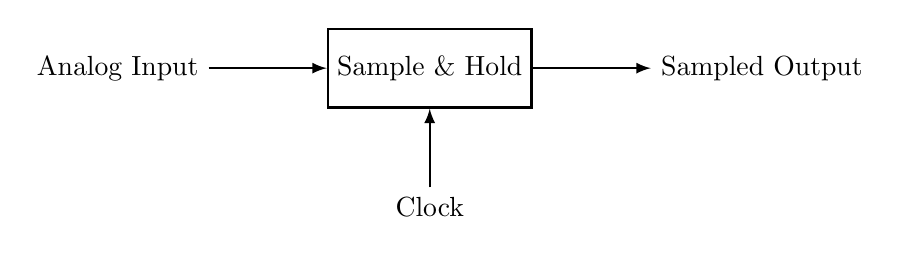
\begin{tikzpicture}[auto, >=latex, thick, node distance=2cm]
    \node (input) {Analog Input};
    \node [draw, rectangle, minimum size=1cm, right=1.5cm of input] (sh) {Sample \& Hold};
    \node [right=1.5cm of sh] (output) {Sampled Output};
    \node [below=1cm of sh] (clock) {Clock};

    \draw [->] (input) -- (sh);
    \draw [->] (sh) -- (output);
    \draw [->] (clock) -- (sh);
\end{tikzpicture}
\captionof{figure}{Sample and Hold Circuit}
\end{center}

\begin{center}
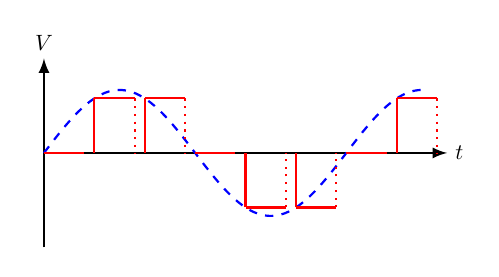
\begin{tikzpicture}[x=0.08cm,y=1.0cm, >=latex, thick, scale=0.8, transform shape]
    \draw[->] (0,0) -- (80,0) node[right] {$t$};
    \draw[->] (0,-1.5) -- (0,1.5) node[above] {$V$};

    \draw[blue, dashed] plot[domain=0:75, samples=100] (\x, {sin(6*\x)});
    \foreach \x in {0, 10, 20, 30, 40, 50, 60, 70} {
        \draw[red, thick] (\x, {sin(6*\x)}) -- (\x+8, {sin(6*\x)});
        \draw[red, thick] (\x, {sin(6*\x)}) -- (\x, 0);
        \draw[red, thick, dotted] (\x+8, {sin(6*\x)}) -- (\x+8, 0);
    }
\end{tikzpicture}
\captionof{figure}{Sample and Hold Waveform}
\end{center}

\begin{itemize}
    \item \textbf{Sampling mode}: Switch closes, capacitor charges to input voltage
    \item \textbf{Hold mode}: Switch opens, capacitor maintains voltage
\end{itemize}
\end{solutionbox}

\begin{mnemonicbox}
\mnemonic{CHASED: Capacitor Holds Amplitude Samples for Extended Duration}
\end{mnemonicbox}

\questionmarks{3(c)}{7}{What is sampling? Explain types of sampling in brief.}

\begin{solutionbox}
\textbf{Sampling} is the process of converting a continuous-time signal into a discrete-time signal by taking measurements at regular intervals.

\begin{center}
\captionof{table}{Types of Sampling}
\begin{tabulary}{\linewidth}{|L|L|L|}
\hline
\textbf{Type} & \textbf{Description} & \textbf{Characteristics} \\ \hline
Natural Sampling & Signal is multiplied with rectangular pulses & Retains original signal shape during pulse \\ \hline
Flat-top Sampling & Sample value is held constant during sampling interval & Creates a staircase-like output \\ \hline
Ideal Sampling & Instantaneous samples represented as impulses & Theoretical concept with zero width pulses \\ \hline
Uniform Sampling & Samples taken at equal time intervals & Most common in practice \\ \hline
Non-uniform Sampling & Samples taken at varying intervals & Used for specialized applications \\ \hline
\end{tabulary}
\end{center}

\begin{center}
\begin{tikzpicture}[x=0.08cm, y=0.8cm, >=latex, thick]
    \node at (-20, 1.5) {Natural};
    \draw[->] (0,0) -- (60,0);
    \foreach \x in {5, 15, ..., 55} {
        \draw[blue, thick] (\x, 0) -- (\x, {sin(6*\x)});
        \draw[blue, thick] (\x+2, 0) -- (\x+2, {sin(6*(\x+2))});
        \draw[blue, thick] (\x, {sin(6*\x)}) -- (\x+2, {sin(6*(\x+2))});
    }

    \node at (-20, -2.5) {Flat-top};
    \draw[->] (0,-4) -- (60,-4);
    \foreach \x in {5, 15, ..., 55} {
        \draw[red, thick] (\x, -4) -- (\x, {sin(6*\x)-4});
        \draw[red, thick] (\x+2, -4) -- (\x+2, {sin(6*\x)-4});
        \draw[red, thick] (\x, {sin(6*\x)-4}) -- (\x+2, {sin(6*\x)-4});
    }
\end{tikzpicture}
\captionof{figure}{Natural vs Flat-top Sampling}
\end{center}

\begin{itemize}
    \item \textbf{Nyquist criterion}: Sampling frequency must be at least twice the highest frequency in the signal
\end{itemize}
\end{solutionbox}

\begin{mnemonicbox}
\mnemonic{INFUN: Ideal, Natural, Flat-top, Uniform, Non-uniform}
\end{mnemonicbox}

\questionmarks{3(a OR)}{3}{Explain quantization process and its necessity.}

\begin{solutionbox}
\textbf{Quantization Process} maps continuous amplitude values to finite discrete levels for digital representation.

\begin{center}
\captionof{table}{Quantization Process and Necessity}
\begin{tabulary}{\linewidth}{|L|L|}
\hline
\textbf{Aspect} & \textbf{Description} \\ \hline
Process & Dividing amplitude range into discrete levels \\ \hline
Necessity & Required for analog-to-digital conversion \\ \hline
Effect & Introduces quantization error/noise \\ \hline
Parameters & Step size, number of levels ($2^n$ for n-bit) \\ \hline
\end{tabulary}
\end{center}

\begin{itemize}
    \item \textbf{Step size calculation}: Step size = $(V_{\max} - V_{\min})/2^n$
    \item \textbf{Quantization error}: Maximum error is $\pm Q/2$ where $Q$ is step size
\end{itemize}
\end{solutionbox}

\begin{mnemonicbox}
\mnemonic{SEND: Step-size Establishes Noise in Digitization}
\end{mnemonicbox}

\questionmarks{3(b OR)}{4}{State and explain Nyquist Criteria for sampling of signal.}

\begin{solutionbox}
\textbf{Nyquist Sampling Theorem} states that to perfectly reconstruct a bandlimited signal, the sampling frequency must be at least twice the highest frequency component in the signal.

\begin{center}
\captionof{table}{Nyquist Criteria}
\begin{tabulary}{\linewidth}{|L|L|}
\hline
\textbf{Parameter} & \textbf{Description} \\ \hline
Criterion & $f_s \ge 2f_{\max}$ \\ \hline
Nyquist Rate & $2f_{\max}$ (minimum sampling frequency) \\ \hline
Nyquist Interval & $1/(2f_{\max})$ (maximum sampling period) \\ \hline
Aliasing & Occurs when $f_s < 2f_{\max}$ \\ \hline
\end{tabulary}
\end{center}

\begin{itemize}
    \item \textbf{Consequences of undersampling}: Aliasing (frequency folding)
    \item \textbf{Practical application}: Anti-aliasing filters used before sampling
\end{itemize}
\end{solutionbox}

\begin{mnemonicbox}
\mnemonic{TRAP-A: Twice Rate Avoids Problematic Aliasing}
\end{mnemonicbox}

\questionmarks{3(c OR)}{7}{Explain PAM, PWM and PPM with waveform.}

\begin{solutionbox}
\begin{center}
\captionof{table}{Pulse Modulation Techniques}
\begin{tabulary}{\linewidth}{|L|L|L|L|}
\hline
\textbf{Technique} & \textbf{Description} & \textbf{Parameter Varied} & \textbf{Application} \\ \hline
PAM & Pulse Amplitude Modulation & Amplitude of pulses & Simple ADC systems \\ \hline
PWM & Pulse Width Modulation & Width/duration of pulses & Motor control, power regulation \\ \hline
PPM & Pulse Position Modulation & Position/timing of pulses & High noise immunity systems \\ \hline
\end{tabulary}
\end{center}

\begin{center}
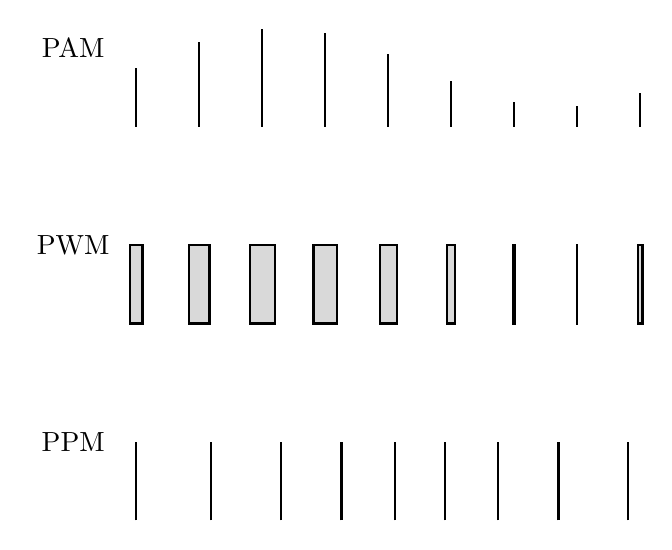
\begin{tikzpicture}[x=0.08cm, y=0.5cm, >=latex, thick]
    \node at (-10, 2) {PAM};
    \foreach \x in {0, 10, ..., 80} {
        \draw[thick] (\x, 0) -- (\x, {1.5 + sin(4*\x)});
    }
    
    \node at (-10, -3) {PWM};
    \foreach \x in {0, 10, ..., 80} {
        \draw[thick, fill=gray!30] ({\x-1-sin(4*\x)}, -5) rectangle ({\x+1+sin(4*\x)}, -3);
    }
    
    \node at (-10, -8) {PPM};
    \foreach \x in {0, 10, ..., 80} {
        \draw[thick] ({\x+sin(4*\x)*3}, -10) -- ({\x+sin(4*\x)*3}, -8);
    }
\end{tikzpicture}
\captionof{figure}{Pulse Modulation Waveforms}
\end{center}

\begin{itemize}
    \item \textbf{PAM}: Simplest form, most susceptible to noise
    \item \textbf{PWM}: Better noise immunity, easy generation
    \item \textbf{PPM}: Best noise immunity, requires precise timing
\end{itemize}
\end{solutionbox}

\begin{mnemonicbox}
\mnemonic{AWP-PAW: Amplitude, Width, Position - Pulse Alteration Ways}
\end{mnemonicbox}


% Q4 Conversion

\questionmarks{4(a)}{3}{What is slope overload noise and granular noise in DM?}

\begin{solutionbox}
\begin{center}
\captionof{table}{Noise Types in Delta Modulation}
\begin{tabulary}{\linewidth}{|L|L|L|L|}
\hline
\textbf{Noise Type} & \textbf{Definition} & \textbf{Cause} & \textbf{Solution} \\ \hline
Slope Overload Noise & Error when signal slope exceeds step size capability & Step size too small for rapidly changing signals & Increase step size or sampling frequency \\ \hline
Granular Noise & Error due to continuous hunting around slowly varying signals & Step size too large for slowly changing signals & Decrease step size \\ \hline
\end{tabulary}
\end{center}

\begin{center}
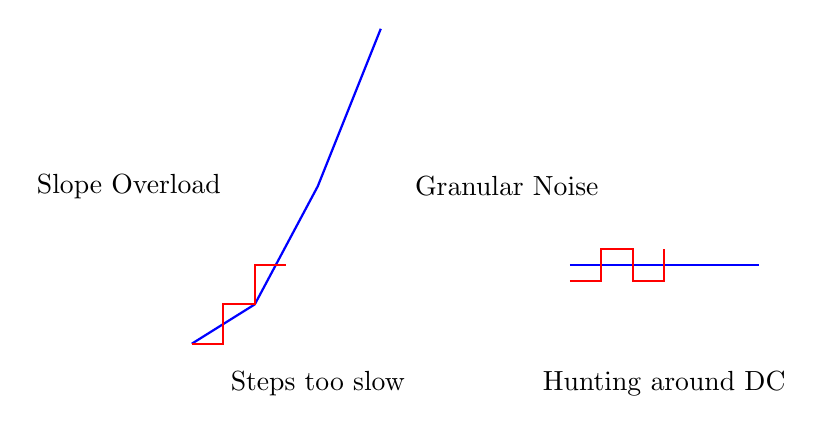
\begin{tikzpicture}[x=0.08cm, y=1.0cm, >=latex, thick]
    \node at (-10, 2) {Slope Overload};
    \draw[blue] (0,0) -- (10,0.5) -- (20,2) -- (30,4);
    \draw[red, step=2] (0,0) -- (5,0) -- (5,0.5) -- (10,0.5) -- (10,1) -- (15,1);
    \node at (20, -0.5) {Steps too slow};

    \node at (50, 2) {Granular Noise};
    \draw[blue] (60,1) -- (90,1);
    \draw[red] (60,0.8) -- (65,0.8) -- (65,1.2) -- (70,1.2) -- (70,0.8) -- (75,0.8) -- (75,1.2);
    \node at (75, -0.5) {Hunting around DC};
\end{tikzpicture}
\captionof{figure}{DM Noise Types}
\end{center}
\end{solutionbox}

\begin{mnemonicbox}
\mnemonic{FAST-SLOW: Fast signals cause Slope overload, SLOW signals cause Granular noise}
\end{mnemonicbox}

\questionmarks{4(b)}{4}{Draw and explain TDM frame.}

\begin{solutionbox}
\begin{center}
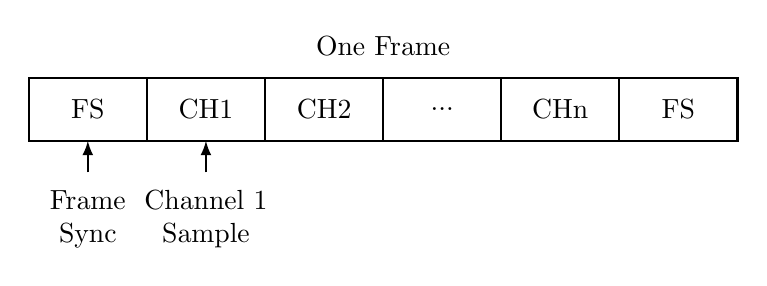
\begin{tikzpicture}[x=1.5cm, y=0.8cm, >=latex, thick]
    \draw (0,0) rectangle (1,1) node[pos=0.5] {FS};
    \draw (1,0) rectangle (2,1) node[pos=0.5] {CH1};
    \draw (2,0) rectangle (3,1) node[pos=0.5] {CH2};
    \draw (3,0) rectangle (4,1) node[pos=0.5] {...};
    \draw (4,0) rectangle (5,1) node[pos=0.5] {CHn};
    \draw (5,0) rectangle (6,1) node[pos=0.5] {FS};
    
    \node at (3, 1.5) {One Frame};
    \draw [->] (0.5, -0.5) -- (0.5, 0) node[below=0.5cm, align=center] {Frame\\Sync};
    \draw [->] (1.5, -0.5) -- (1.5, 0) node[below=0.5cm, align=center] {Channel 1\\Sample};
\end{tikzpicture}
\captionof{figure}{TDM Frame Structure}
\end{center}

\begin{center}
\captionof{table}{TDM Frame Components}
\begin{tabulary}{\linewidth}{|L|L|}
\hline
\textbf{Component} & \textbf{Description} \\ \hline
Frame Sync (FS) & Pattern that marks the start of frame \\ \hline
Time Slot & Portion allocated to one channel \\ \hline
Channel Sample & Data from a specific channel \\ \hline
Frame Length & Total duration (FS + all channels) \\ \hline
\end{tabulary}
\end{center}

\begin{itemize}
    \item \textbf{Working principle}: Allocates different time slots to different channels
    \item \textbf{Synchronization}: Essential for proper demultiplexing
\end{itemize}
\end{solutionbox}

\begin{mnemonicbox}
\mnemonic{FAST-Ch: Frame And Slots for Transmitting Channels}
\end{mnemonicbox}

\questionmarks{4(c)}{7}{Describe the function of each block of PCM transmitter and Receiver. Give application, advantage and disadvantage of PCM system.}

\begin{solutionbox}
\begin{center}
\begin{tikzpicture}[node distance=1.5cm, auto, >=latex, thick, scale=0.8, transform shape]
    % Transmitter
    \node [gtu block] (samp) {Sampler};
    \node [gtu block, right=1cm of samp] (quant) {Quantizer};
    \node [gtu block, right=1cm of quant] (enc) {Encoder};
    \node [gtu block, right=1cm of enc] (lc) {Line Coder};
    
    % Receiver
    \node [gtu block, below=2cm of lc] (ld) {Line Decoder};
    \node [gtu block, left=1cm of ld] (dec) {Decoder};
    \node [gtu block, left=1cm of dec] (filt) {Reconstruction\\Filter};
    
    \node at ($(enc)!0.5!(dec)$) [yshift=0.5cm] {PCM Transmitter};
    \node at ($(ld)!0.5!(filt)$) [yshift=-1cm] {PCM Receiver};
    
    \draw [gtu arrow] (samp) -- (quant);
    \draw [gtu arrow] (quant) -- (enc);
    \draw [gtu arrow] (enc) -- (lc);
    \draw [gtu arrow, dashed] (lc) -- (ld) node[midway, right] {Channel};
    \draw [gtu arrow] (ld) -- (dec);
    \draw [gtu arrow] (dec) -- (filt);
\end{tikzpicture}
\captionof{figure}{PCM System}
\end{center}

\begin{center}
\captionof{table}{PCM Block Functions}
\begin{tabulary}{\linewidth}{|L|L|}
\hline
\textbf{Block} & \textbf{Function} \\ \hline
Sampler & Converts analog signal to PAM signal \\ \hline
Quantizer & Assigns discrete levels to samples \\ \hline
Encoder & Converts quantized levels to binary code \\ \hline
Line Coder & Converts binary to transmission format \\ \hline
Line Decoder & Recovers binary from received signal \\ \hline
Decoder & Converts binary back to quantized levels \\ \hline
Reconstruction Filter & Smooths decoded output into analog signal \\ \hline
\end{tabulary}
\end{center}

\textbf{Applications, Advantages and Disadvantages:}

\begin{center}
\captionof{table}{PCM System Characteristics}
\begin{tabulary}{\linewidth}{|L|L|}
\hline
\textbf{Category} & \textbf{Description} \\ \hline
Applications & Telephone systems, CD audio, Digital TV, Mobile communications \\ \hline
Advantages & Immune to noise, Signal regeneration possible, Compatible with digital systems \\ \hline
Disadvantages & Requires higher bandwidth, Higher complexity, Quantization noise \\ \hline
\end{tabulary}
\end{center}
\end{solutionbox}

\begin{mnemonicbox}
\mnemonic{SEQUEL-DR: Sample, Quantize, Encode - Line code, Decode, Reconstruct}
\end{mnemonicbox}

\questionmarks{4(a OR)}{3}{Give difference between DM and ADM modulation.}

\begin{solutionbox}
\begin{center}
\captionof{table}{Comparison between DM and ADM}
\begin{tabulary}{\linewidth}{|L|L|L|}
\hline
\textbf{Parameter} & \textbf{Delta Modulation (DM)} & \textbf{Adaptive Delta Modulation (ADM)} \\ \hline
Step Size & Fixed & Variable (adapts to signal slope) \\ \hline
Tracking Ability & Limited & Better signal tracking \\ \hline
Noise Performance & Suffers from slope overload and granular noise & Reduced noise problems \\ \hline
Complexity & Simpler & More complex \\ \hline
\end{tabulary}
\end{center}

\begin{center}
\begin{tikzpicture}[x=0.08cm, y=0.5cm, >=latex, thick]
    \node at (-15, 0) {Input};
    \draw[dashed] plot[domain=0:50] (\x, {sin(6*\x)*3});
    
    \node at (-15, -4) {DM Output};
    \draw[red] (0,-4) -- (2,-3.5) -- (4,-4) -- (6,-3.5);
    \node at (60, -4) {Fixed steps};
    
    \node at (-15, -8) {ADM Output};
    \draw[blue] (0,-8) -- (2,-7) -- (4,-5) -- (6,-8);
    \node at (60, -8) {Variable steps};
\end{tikzpicture}
\captionof{figure}{DM vs ADM Tracking}
\end{center}
\end{solutionbox}

\begin{mnemonicbox}
\mnemonic{FAST-VAR: Fixed And Simple Tracking vs Variable Adaptive Response}
\end{mnemonicbox}

\questionmarks{4(b OR)}{4}{Explain Block diagram of basic PCM-TDM system.}

\begin{solutionbox}
\begin{center}
\begin{tikzpicture}[node distance=1.5cm, auto, >=latex, thick, scale=0.75, transform shape]
    \node (in1) {Input 1};
    \node [right=1cm of in1, gtu block] (lpf1) {LPF};
    
    \node [below=0.5cm of in1] (in2) {Input 2};
    \node [right=1cm of in2, gtu block] (lpf2) {LPF};
    
    \node [below=0.5cm of in2] (inn) {Input n};
    \node [right=1cm of inn, gtu block] (lpfn) {LPF};
    
    \node [gtu block, right=3cm of lpf2, minimum height=3cm] (mux) {Multiplexer};
    
    \draw [gtu arrow] (in1) -- (lpf1);
    \draw [gtu arrow] (in2) -- (lpf2);
    \draw [gtu arrow] (inn) -- (lpfn);
    
    \draw [gtu arrow] (lpf1) -- (mux.west |- lpf1.east);
    \draw [gtu arrow] (lpf2) -- (mux.west |- lpf2.east);
    \draw [gtu arrow] (lpfn) -- (mux.west |- lpfn.east);
    
    \node [gtu block, right=1cm of mux] (enc) {PCM Encoder};
    \draw [gtu arrow] (mux) -- (enc);
    
    \node [right=2cm of enc] (out) {Channel};
    \draw [gtu arrow] (enc) -- (out);
\end{tikzpicture}
\captionof{figure}{PCM-TDM System}
\end{center}

\begin{center}
\captionof{table}{PCM-TDM System Components}
\begin{tabulary}{\linewidth}{|L|L|}
\hline
\textbf{Component} & \textbf{Function} \\ \hline
Low-pass Filters & Limit bandwidth of input signals \\ \hline
Multiplexer & Combines multiple signals into time slots \\ \hline
PCM Encoder & Converts to digital (sample, quantize, encode) \\ \hline
Transmission Channel & Carries digitized, multiplexed signal \\ \hline
PCM Decoder & Reconstructs quantized samples \\ \hline
Demultiplexer & Separates channels from time slots \\ \hline
\end{tabulary}
\end{center}

\begin{itemize}
    \item \textbf{Working principle}: Combines time division multiplexing with pulse code modulation
\end{itemize}
\end{solutionbox}

\begin{mnemonicbox}
\mnemonic{FLIMPED: Filter, Limit, Multiplex, PCM Encode, Decode}
\end{mnemonicbox}

\questionmarks{4(c OR)}{7}{Explain DPCM modulator with equation and waveform.}

\begin{solutionbox}
\textbf{Differential Pulse Code Modulation (DPCM)} encodes the difference between the current sample and a predicted value based on previous samples.

\textbf{Equation:}
\begin{itemize}
    \item Error signal: $e(n) = x(n) - \hat{x}(n)$
    \item Where $x(n)$ is current sample, $\hat{x}(n)$ is predicted sample
    \item Prediction: $\hat{x}(n) = \Sigma(a_i \times x(n-i))$
    \item Transmitted signal: DPCM output $= Q[e(n)]$
\end{itemize}

\begin{center}
\begin{tikzpicture}[node distance=2cm, auto, >=latex, thick]
    \node (input) {$x(n)$};
    \node [draw, circle, right=1cm of input] (sum) {+};
    \node [gtu block, right=1cm of sum] (quant) {Quantizer};
    \node [gtu block, right=1cm of quant] (enc) {Encoder};
    \node [right=1cm of enc] (out) {Output};
    
    \node [gtu block, below=1cm of quant] (pred) {Predictor};
    \node [draw, circle, left=1cm of pred] (sub) {+}; % Feedback summation
    
    \draw [gtu arrow] (input) -- (sum);
    \draw [gtu arrow] (sum) -- (quant);
    \draw [gtu arrow] (quant) -- (enc);
    \draw [gtu arrow] (enc) -- (out);
    
    \draw [gtu arrow] (quant) |- (sub);
    \draw [gtu arrow] (sub) -- (pred);
    \draw [gtu arrow] (pred) -| (sum) node[pos=0.9, left] {-};
    \draw [gtu arrow] (pred) -| (sub) node[pos=0.9, left] {+};
\end{tikzpicture}
\captionof{figure}{DPCM Modulator}
\end{center}

\begin{center}
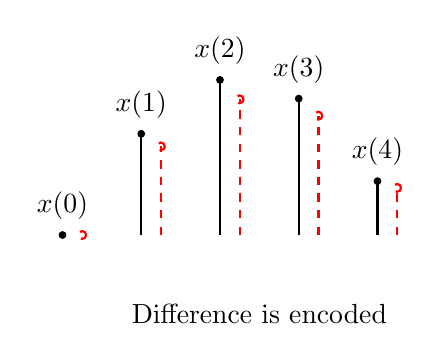
\begin{tikzpicture}[x=0.5cm, y=0.5cm, >=latex, thick]
    \foreach \x in {0,1,2,3,4} {
        \draw[thick] (\x*2, 0) -- (\x*2, {sin(20*\x*2)*4}) node[circle, fill, inner sep=1pt, label=above:$x(\x)$] {};
    }
    \foreach \x in {0,1,2,3,4} {
        \draw[dashed, red] (\x*2+0.5, 0) -- (\x*2+0.5, {sin(20*\x*2)*3.5}) node[circle, draw, red, inner sep=1pt] {};
    }
    \node at (5, -2) {Difference is encoded};
\end{tikzpicture}
\captionof{figure}{DPCM Waveform}
\end{center}

\begin{center}
\captionof{table}{DPCM Characteristics}
\begin{tabulary}{\linewidth}{|L|L|}
\hline
\textbf{Feature} & \textbf{Description} \\ \hline
Advantage & Reduced bit rate (30-50\% compared to PCM) \\ \hline
Prediction & Uses previous sample(s) for current prediction \\ \hline
Complexity & Higher than PCM but lower than ADPCM \\ \hline
Application & Speech coding, image compression \\ \hline
\end{tabulary}
\end{center}
\end{solutionbox}

\begin{mnemonicbox}
\mnemonic{PQED: Predict, Quantize Error, Encode Difference}
\end{mnemonicbox}

% Q5 Conversion

\questionmarks{5(a)}{3}{Define Antenna and radiation pattern and polarization.}

\begin{solutionbox}
\begin{center}
\captionof{table}{Antenna Definitions}
\begin{tabulary}{\linewidth}{|L|L|}
\hline
\textbf{Term} & \textbf{Definition} \\ \hline
Antenna & A device that converts electrical energy into electromagnetic waves and vice versa \\ \hline
Radiation Pattern & Graphical representation of radiation properties of an antenna as a function of space coordinates \\ \hline
Polarization & Orientation of the electric field vector of the electromagnetic wave radiated by the antenna \\ \hline
\end{tabulary}
\end{center}

\textbf{Types of Polarization:}
\begin{itemize}
    \item \textbf{Linear}: Electric field oscillates in one direction (vertical, horizontal)
    \item \textbf{Circular}: Electric field rotates with constant amplitude (RHCP, LHCP)
    \item \textbf{Elliptical}: Electric field rotates with varying amplitude
\end{itemize}
\end{solutionbox}

\begin{mnemonicbox}
\mnemonic{WAVE-PRO: Wireless Antenna Validates Electromagnetic Propagation, Radiation, Orientation}
\end{mnemonicbox}

\questionmarks{5(b)}{4}{Explain Microstrip Antenna with sketch.}

\begin{solutionbox}
\begin{center}
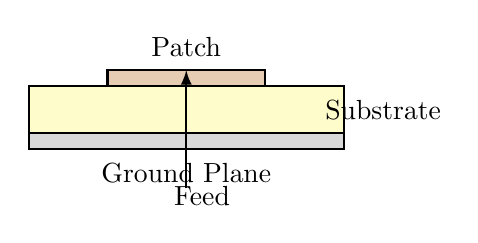
\begin{tikzpicture}[x=1cm, y=1cm, >=latex, thick]
    % Ground
    \fill[gray!30] (0,0) rectangle (4,0.2);
    \draw (0,0) rectangle (4,0.2);
    \node at (2, -0.3) {Ground Plane};
    
    % Substrate
    \fill[yellow!20] (0,0.2) rectangle (4,0.8);
    \draw (0,0.2) rectangle (4,0.8);
    \node at (4.5, 0.5) {Substrate};
    
    % Patch
    \fill[brown!40] (1,0.8) rectangle (3,1.0);
    \draw (1,0.8) rectangle (3,1.0);
    \node at (2, 1.3) {Patch};
    
    % Feed
    \draw[->] (2, -0.5) -- (2, 1.0);
    \node at (2.2, -0.6) {Feed};
\end{tikzpicture}
\captionof{figure}{Microstrip Patch Antenna}
\end{center}

\begin{center}
\captionof{table}{Microstrip Antenna Components}
\begin{tabulary}{\linewidth}{|L|L|}
\hline
\textbf{Component} & \textbf{Function} \\ \hline
Patch & Radiating element (usually copper) \\ \hline
Substrate & Dielectric material between patch and ground \\ \hline
Ground Plane & Metal layer at bottom \\ \hline
Feed Point & Connection point for signal \\ \hline
\end{tabulary}
\end{center}

\begin{itemize}
    \item \textbf{Working principle}: Fringing fields at edges cause radiation
    \item \textbf{Advantages}: Low profile, lightweight, easy fabrication, compatible with PCB
\end{itemize}
\end{solutionbox}

\begin{mnemonicbox}
\mnemonic{SPGF: Substrate, Patch, Ground, Feed}
\end{mnemonicbox}

\questionmarks{5(c)}{7}{Explain delta modulation with necessary sketch and waveform.}

\begin{solutionbox}
Delta Modulation (DM) is the simplest form of differential pulse code modulation where the difference between successive samples is encoded into a single bit.

\begin{center}
\begin{tikzpicture}[node distance=2cm, auto, >=latex, thick]
    \node (input) {Input};
    \node [draw, circle, right=1cm of input] (sum) {+};
    \node [gtu block, right=1cm of sum] (quant) {1-bit\\Quantizer};
    \node [right=1cm of quant] (out) {Output};
    
    \node [gtu block, below=1cm of quant] (int) {Integrator};
    \node [gtu block, left=1cm of int] (delay) {Delay};
    
    \draw [gtu arrow] (input) -- (sum);
    \draw [gtu arrow] (sum) -- (quant);
    \draw [gtu arrow] (quant) -- (out);
    
    \draw [gtu arrow] (quant) |- (delay);
    \draw [gtu arrow] (delay) -- (int);
    \draw [gtu arrow] (int) -| (sum) node[pos=0.9, left] {-};
\end{tikzpicture}
\captionof{figure}{Delta Modulator}
\end{center}

\begin{center}
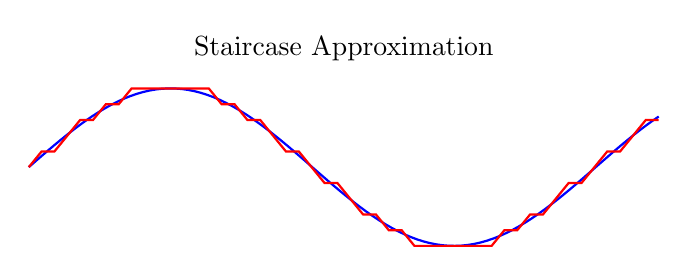
\begin{tikzpicture}[x=0.08cm, y=1.0cm, >=latex, thick]
    \draw[blue, thick] plot[domain=0:100, samples=100] (\x, {sin(4*\x)});
    \draw[red, thick, step=0.2] plot[domain=0:100, samples=50] (\x, {round(sin(4*\x)/0.2)*0.2});
    \node at (50, 1.5) {Staircase Approximation};
\end{tikzpicture}
\captionof{figure}{Delta Modulation Waveform}
\end{center}

\begin{center}
\captionof{table}{Delta Modulation Characteristics}
\begin{tabulary}{\linewidth}{|L|L|}
\hline
\textbf{Characteristic} & \textbf{Description} \\ \hline
Bit Rate & 1 bit per sample \\ \hline
Step Size & Fixed (major limitation) \\ \hline
Slope Overload & Occurs when signal changes faster than step size can track \\ \hline
Granular Noise & Occurs in slowly changing signals (continuous hunting) \\ \hline
Advantages & Simplicity, low bit rate \\ \hline
Disadvantages & Limited dynamic range, noise problems \\ \hline
\end{tabulary}
\end{center}
\end{solutionbox}

\begin{mnemonicbox}
\mnemonic{SIGN-UP: SInGle bit, Next step Up or down, Predict}
\end{mnemonicbox}

\questionmarks{5(a OR)}{3}{What is smart antenna? list application of it.}

\begin{solutionbox}
A \textbf{Smart Antenna} is an adaptive array system that uses digital signal processing algorithms to dynamically adjust its radiation pattern to enhance communication performance.

\begin{center}
\captionof{table}{Smart Antenna Applications}
\begin{tabulary}{\linewidth}{|L|L|}
\hline
\textbf{Application} & \textbf{Benefit} \\ \hline
Cellular Base Stations & Increased capacity and coverage \\ \hline
Wireless LAN & Improved throughput and reduced interference \\ \hline
Satellite Communications & Better signal quality and power efficiency \\ \hline
Military Communications & Enhanced security and jam resistance \\ \hline
IoT Networks & Extended battery life, improved connectivity \\ \hline
\end{tabulary}
\end{center}

\begin{itemize}
    \item \textbf{Working principle}: Uses beamforming to focus signal energy toward desired users
    \item \textbf{Types}: Switched beam systems and adaptive array systems
\end{itemize}
\end{solutionbox}

\begin{mnemonicbox}
\mnemonic{SWIM-CM: Smart Wireless In Mobile-Cellular-Military}
\end{mnemonicbox}

\questionmarks{5(b OR)}{4}{Explain parabolic reflector antenna With Sketch.}

\begin{solutionbox}
\begin{center}
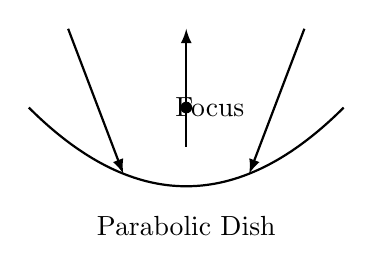
\begin{tikzpicture}[x=1cm, y=1cm, >=latex, thick]
    \draw [domain=-2:2, samples=100] plot (\x, {0.25*\x*\x});
    \draw [->] (-1.5, 2) -- (-0.8, 0.16);
    \draw [->] (1.5, 2) -- (0.8, 0.16);
    \draw [->] (0, 0.5) -- (0, 2);
    
    \node [circle, fill, inner sep=1.5pt] at (0, 1) {};
    \node at (0.3, 1) {Focus};
    
    \node at (0, -0.5) {Parabolic Dish};
\end{tikzpicture}
\captionof{figure}{Parabolic Reflector Antenna}
\end{center}

\begin{center}
\captionof{table}{Parabolic Reflector Components}
\begin{tabulary}{\linewidth}{|L|L|}
\hline
\textbf{Component} & \textbf{Function} \\ \hline
Parabolic Dish & Reflects and focuses signals \\ \hline
Feed Horn & Radiates/receives signals at focal point \\ \hline
Supporting Structure & Maintains geometry and stability \\ \hline
Waveguide & Connects feed horn to transmitter/receiver \\ \hline
\end{tabulary}
\end{center}

\begin{itemize}
    \item \textbf{Working principle}: Incoming parallel rays are reflected to focus at focal point
    \item \textbf{Characteristics}: High gain, directivity, narrow beamwidth
    \item \textbf{Applications}: Satellite communication, radio astronomy, radar, microwave links
\end{itemize}
\end{solutionbox}

\begin{mnemonicbox}
\mnemonic{PFGH: Parabolic Focus Gives High-gain}
\end{mnemonicbox}

\questionmarks{5(c OR)}{7}{Explain Adaptive Delta modulation with necessary sketch and waveform.}

\begin{solutionbox}
Adaptive Delta Modulation (ADM) improves on standard DM by dynamically adjusting the step size according to the input signal characteristics.

\begin{center}
\begin{tikzpicture}[node distance=2cm, auto, >=latex, thick]
    \node (input) {Input};
    \node [draw, circle, right=1cm of input] (sum) {+};
    \node [gtu block, right=1cm of sum] (quant) {1-bit\\Quantizer};
    \node [right=1cm of quant] (out) {Output};
    
    \node [gtu block, below=1cm of quant] (step) {Step Size\\Control};
    \node [gtu block, below=1cm of step] (int) {Integrator};
    
    \draw [gtu arrow] (input) -- (sum);
    \draw [gtu arrow] (sum) -- (quant);
    \draw [gtu arrow] (quant) -- (out);
    
    \draw [gtu arrow] (quant) -- (step);
    \draw [gtu arrow] (step) -- (int);
    \draw [gtu arrow] (int) -| (sum) node[pos=0.9, left] {-};
\end{tikzpicture}
\captionof{figure}{Adaptive Delta Modulator}
\end{center}

\begin{center}
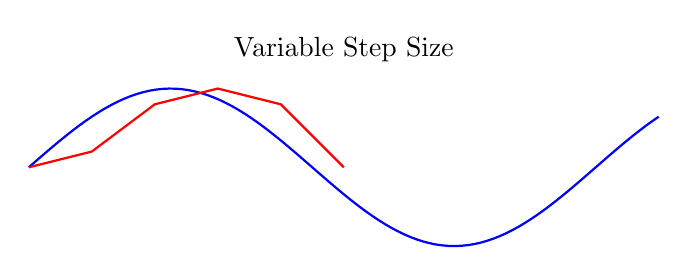
\begin{tikzpicture}[x=0.08cm, y=1.0cm, >=latex, thick]
    \draw[blue, thick] plot[domain=0:100, samples=100] (\x, {sin(4*\x)});
    \draw[red, thick] (0,0) -- (10,0.2) -- (20,0.8) -- (30,1.0) -- (40,0.8) -- (50,0);
    \node at (50, 1.5) {Variable Step Size};
\end{tikzpicture}
\captionof{figure}{ADM Waveform}
\end{center}

\begin{center}
\captionof{table}{ADM Characteristics}
\begin{tabulary}{\linewidth}{|L|L|}
\hline
\textbf{Aspect} & \textbf{Description} \\ \hline
Step Size & Variable (adapts to signal slope) \\ \hline
Control Logic & Increases step size for consecutive same bits \\ \hline
Advantages & Reduced slope overload and granular noise \\ \hline
Disadvantages & More complex than DM \\ \hline
\end{tabulary}
\end{center}

\begin{itemize}
    \item \textbf{Step size adaptation}: $\mu(n) = \mu(n-1) \times K$ if consecutive bits are same
    \item \textbf{Step size adaptation}: $\mu(n) = \mu(n-1) / K$ if consecutive bits change
\end{itemize}
\end{solutionbox}

\begin{mnemonicbox}
\mnemonic{ADVISED: ADaptive Variable Increment Step for Enhanced Delta modulation}
\end{mnemonicbox}

\end{document}

